
\section*{№ 4.20}
\begin{mdframed}
	На вiдрiзку $AB$ довжиною $l$ навмання вибрано точку $O$.\\ 
	Знайдiть ймовiрнiсть того, що вiдношення $|AO| / |AB|$ не перевищує $0.6$.
\end{mdframed}

Тобто,
$$
\begin{tikzpicture}
	\draw (0,0) node[anchor=east] {A}
		-- (4,0) node[anchor=west] {B};
	\filldraw[black] (1,0) circle (2pt) node[anchor=north] {O};
\end{tikzpicture}
$$

Маємо:
$$ \Omega = [0;1];\quad x \in \Omega \text{ - координата точки } O $$
$$ \text{Подія } A = \{ |AO| / |AB| \le 0.6\} = 
\{ x \le 0.6 \} $$
$$ P(A) = \frac{\mu(A)}{\mu(\Omega)} = \frac{0.6}{1} = 0.6 $$

\begin{mdframed}[style=ans]
	$$ P(A) = 0.6 $$
\end{mdframed}


\section*{№ 4.21}
\begin{mdframed}
	На вiдрiзку [−1, 2] навмання вибрано двi точки A i B. Знайдiть ймовiрнiсть
того, що вiдстань мiж ними виявиться меншою за 2 i точка A лежатиме лiвiше
одиницi.
\end{mdframed}

Тобто,
$$
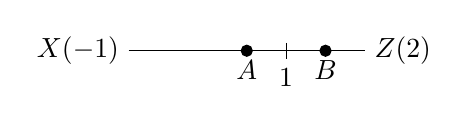
\begin{tikzpicture}
	\draw (-1,0) node[anchor=east] {$X(-1)$}
		-- (2,0) node[anchor=west] {$Z(2)$};
	\filldraw[black] (0.5,0) circle (2pt) node[anchor=north] {$A$};
	\filldraw[black] (1.5,0) circle (2pt) node[anchor=north] {$B$};
	\draw (1,0.1) -- (1,-0.1) node[anchor=north] {$1$};
\end{tikzpicture}
$$

Маємо:
$$ \Omega = [-1;2]^2;\quad (a,b) \in \Omega \text{ - координати точок $A$ та $B$} $$
$$ \text{Подія } A = \{ |b-a| < 2 \;\&\; a<1 \};\quad P(A) \text{ - ?}$$

\begin{multicols}{2}
	$$ \begin{cases}
		& b < a + 2 \quad (\text{if } b \ge a) \\
		& b > a - 2 \quad (\text{if } b < a) \\
		& a < 1
	\end{cases}$$
	\columnbreak
	$$
	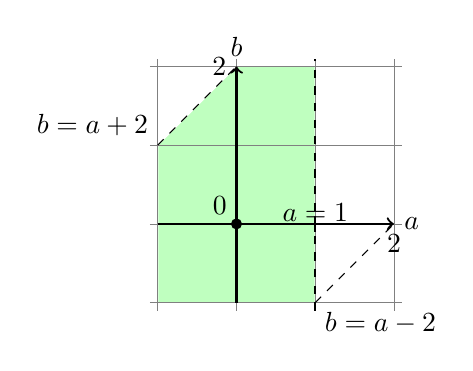
\begin{tikzpicture}
		\filldraw[fill=green!25, draw=black!0] (-1,-1) -- (-1,1) -- (0,2) -- (1,2) -- (1,-1) -- cycle;
		\draw[step=1cm,gray,very thin] (-1.1,-1.1) grid (2.1,2.1);
		\draw[thick,->] (-1,0) -- (2,0) node[anchor=west] {$a$} node[below] {$2$};
		\fill (0,0) circle (2pt) node[above left] {$0$};
		\draw[thick,->] (0,-1) -- (0,2) node[anchor=south] {$b$} node[left] {$2$};
		\draw[thick,dashed] (1, -1.1) -- (1, 2.1);
		\draw[thick] (1, 0.1) -- (1, -0.1) node[anchor=south] {$a = 1$};
		% \draw[thick, dashed] (-1,-1) -- (2,2) node[anchor=west] {$a = b$};
		\draw[dashed] (-1,1) node[anchor=south east] {$b = a+2$}-- (0, 2);
		\draw[dashed] (1,-1) node[anchor=north west] {$b = a-2$} -- (2, 0);
	\end{tikzpicture}
	$$
\end{multicols}

\begin{mdframed}[style=ans]
	$$P(A) = \frac{5.5}{9} = \frac{11}{18}$$
\end{mdframed}


\section*{№ 4.22}
\begin{mdframed}
	Точку (ξ, η) навмання вибрано в квадратi $[0, 1]^2$. 
	Для фiксованого z $\in$ (0, 1) обчислiть ймовiрності
	\begin{enumerate}
		\item P(ξ + 2η < z);
		\item P(max(ξ, η) < z);
		\item P(ξη < z).
	\end{enumerate}
\end{mdframed}

\begin{enumerate}
	\item P(ξ + 2η < z);
		$$\eta < - \frac{\xi}{2} + \frac{z}{2}$$
		$$
		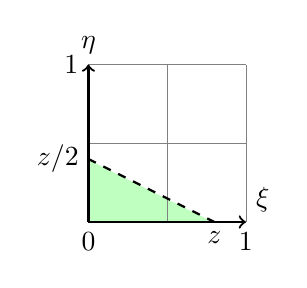
\begin{tikzpicture}
			\filldraw[fill=green!25, draw=black!0] (0,0) -- (0,0.8) node[anchor=east] {$z/2$} -- (1.6,0) node[anchor=north] {$z$} -- cycle;
			\draw[step=1cm,gray,very thin] (0,0) grid (2,2);
			\draw[thick,->] (0,0) node[anchor=north] {$0$} -- (2,0) node[anchor=south west] {$\xi$} node[anchor=north] {$1$};
			\draw[thick,->] (0,0) -- (0,2) node[anchor=south] {$\eta$} node[left] {$1$};
			\draw[thick,dashed] (0, 0.8) -- (1.6, 0);
			% \draw[thick] (1, 0.1) -- (1, -0.1) node[anchor=south] {$a = 1$};
			% \draw[thick, dashed] (-1,-1) -- (2,2) node[anchor=west] {$a = b$};
			% \draw[dashed] (-1,1) node[anchor=south east] {$b = a+2$}-- (0, 2);
			% \draw[dashed] (1,-1) node[anchor=north west] {$b = a-2$} -- (2, 0);
		\end{tikzpicture}
		$$
		$$\mu(A) = \frac{1}{2} (z \cdot \frac{z}{2}) = \frac{z^2}{4}
		\quad\mu(\Omega) = 1$$
		\begin{mdframed}[style=ans]
			$$P(A) = \frac{z^2}{4}$$
		\end{mdframed}

	\item P(max(ξ, η) < z);
		$$\begin{cases}
			\eta > \xi \implies \eta < z \\
			\eta \le \xi \implies \xi < z 	
		\end{cases}$$
		$$
		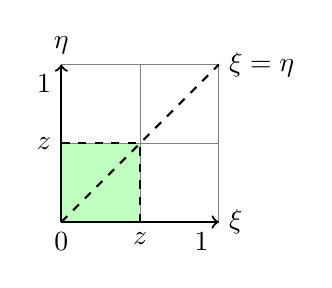
\begin{tikzpicture}
			\filldraw[fill=green!25, draw=black!0] (0,0) rectangle (1,1);
			\draw[step=1cm,gray,very thin] (0,0) grid (2,2);
			\draw[thick,->] (0,0) node[anchor=north] {$0$} -- (2,0) node[anchor=west] {$\xi$} node[anchor=north east] {$1$};
			\draw[thick,->] (0,0) -- (0,2) node[anchor=south] {$\eta$} node[anchor=north east] {$1$};
			\draw[thick,dashed] (0, 0) -- (2, 2) node[anchor=west] {$\xi = \eta$};
			\draw[thick, dashed] (0,1) node[anchor=east] {$z$} -- (1,1); 
			\draw[thick, dashed] (1,0) node[anchor=north] {$z$} -- (1,1); 
		\end{tikzpicture}
		$$
		$$\mu(A) = z^2
		\quad\mu(\Omega) = 1$$
		\begin{mdframed}[style=ans]
			$$P(A) = z^2$$
		\end{mdframed}

	\item P(ξη < z).
		$$\eta < \frac{z}{\xi} \text{ - гіпербола}$$
		$$
		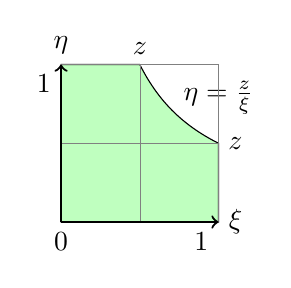
\begin{tikzpicture}
			\filldraw [fill=green!25, draw=black] 
				(1,2) node[anchor=south] {$z$} --
				plot[
					scale=2,
					samples=100,
					domain=0.5:1,
				] (\x,{0.5/(\x)}) -- (2,1) node[right] {$z$} node[above=0.25cm] {$\eta = \frac{z}{\xi}$}
				-- (2,0) -- (0,0) -- (0,2) -- cycle;
			\draw[step=1cm,gray,very thin] (0,0) grid (2,2);
			\draw[thick,->] (0,0) node[anchor=north] {$0$} -- (2,0) node[anchor=west] {$\xi$} node[anchor=north east] {$1$};
			\draw[thick,->] (0,0) -- (0,2) node[anchor=south] {$\eta$} node[anchor=north east] {$1$};
				
		\end{tikzpicture}
		$$
		$$ \mu(A) = z \cdot 1 + \int_z^1 \frac{z}{\xi} d\xi = 
		z + \left. z (1+\ln \xi)\right|_z^1 = z + z (1 + \ln 1 - 1 - \ln z) = z (1 + \ln \frac{1}{z})\quad
		\mu(\Omega) = 1 $$

		\begin{mdframed}[style=ans]
			$$P(A) = z (1 + \ln \frac{1}{z}) = z (1 - \ln z)$$
		\end{mdframed}
\end{enumerate}

\section*{№ 4.23}
\begin{mdframed}
	На колi навмання вибрано три точки A, B i C. Знайдiть ймовiрнiсть того, що
	трикутник ABC виявиться:
	а) тупокутним;
	б) рiвнобедренним
\end{mdframed}
\begin{enumerate}
	\item тупокутний;
	$$\Omega = \{(b,c) \in [0,2\pi]^2 | b < c\}$$
	$b, c$ - Координати точок на дузі кола. 
	Фіксуємо одну точку (А). Дві інші (B,C) вибираємо так, щоб B < C
	\begin{multicols}{2}
		$$
		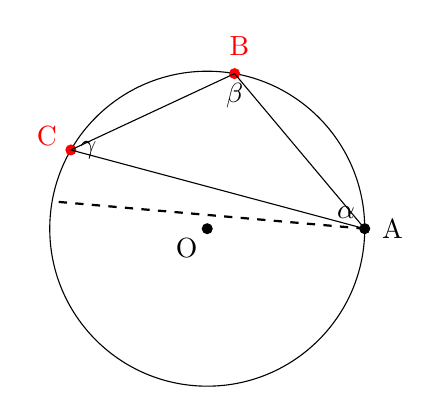
\begin{tikzpicture}
			\coordinate (O) at (0,0);
			\def\R{2};
			\draw (O) circle[radius=\R];
			\fill (O) circle[radius=2pt] node[below left] {O};
			\path (O) ++(0:\R) coordinate (A) node[above left] {$\alpha$};
			\path (O) ++(80:\R) coordinate (B) node[below] {$\beta$};
			\path (O) ++(150:\R) coordinate (C) node[right] {$\gamma$};
			\path (O) ++(170:\R) coordinate (D);
			\fill[black] (A) circle[radius=2pt] ++(0:1em) node {A};
			\fill[red] (B) circle[radius=2pt] ++(80:1em) node {B};
			\fill[red] (C) circle[radius=2pt] ++(150:1em) node {C};
			\draw (A) -- (B) -- (C) -- cycle;
			\draw[thick,dashed] (A) -- (D);
			
		\end{tikzpicture}
		$$
		\columnbreak

		Звернімо увагу, що
		$$
		\begin{cases}
			\alpha = \frac{c - b}{2} \\
			\beta = \frac{2\pi - c}{2} = \pi - \frac{c}{2}\\
			\gamma = \frac{b}{2}
		\end{cases}
		$$
	\end{multicols} 

	$$
	A = \{ (b,c) \in \Omega \;|\;
	\left[\begin{array}{c}
		\alpha > \pi/2 \\
		\beta > \pi/2 \\
		\gamma > \pi/2 \\
	\end{array}\right. \} \implies
	\left[\begin{array}{c}
		c-b > \pi \\
		2\pi - c > \pi \\
		b > \pi \\
	\end{array}\right. \implies
	\left[\begin{array}{c}
		c > b + \pi \\
		c < \pi \\
		b > \pi \\
	\end{array}\right.
	$$
	\pagebreak
	\begin{multicols}{2}
		$$
		\left[\begin{array}{c}
			c > b + \pi \\
			c < \pi \\
			b > \pi \\
		\end{array}\right.
		$$
		\columnbreak
		$$
		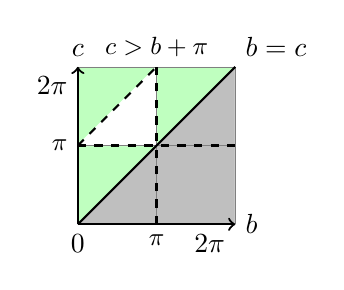
\begin{tikzpicture}
			\filldraw[fill=green!25, draw=black!0] (0,1) -- (0,2) -- (1,2) -- cycle;
			\filldraw[fill=green!25, draw=black!0] (0,0) -- (0,1) -- (1,1) -- cycle;
			\filldraw[fill=green!25, draw=black!0] (1,1) -- (1,2) -- (2,2) -- cycle;
			\filldraw[fill=black!25, draw=black!0] (0,0) -- (2,2) -- (2,0) -- cycle;
			\draw[step=1cm,gray,very thin] (0,0) grid (2,2);
			\draw[thick,->] (0,0) node[anchor=north] {$0$} -- (2,0) node[anchor=west] {$b$} node[anchor=north east] {$2\pi$};
			\draw[thick,->] (0,0) -- (0,2) node[anchor=south] {$c$} node[anchor=north east] {$2\pi$};
			\draw[thick] (0,0) -- (2,2) node[above right] {$b=c$};
			\draw[thick, dashed] (1,0) node[below] {\small $\pi$} -- (1,2); 
			\draw[thick, dashed] (0,1) node[left] {\small $\pi$} -- (2,1); 
			\draw[thick, dashed] (0,1) -- (1,2) node[above] {\small $c > b + \pi$}; 
		\end{tikzpicture}
		$$
	\end{multicols}

	$$\mu(\Omega) = \frac{1}{2} (2\pi)^2 = 2\pi^2;\quad
	\mu(A) = \frac{3}{4} \cdot \frac{4\pi^2}{2} = \frac{3}{4} 2\pi^2 \cdot $$
	\begin{mdframed}[style=ans]
		$$P(A) = \frac{\frac{3}{4} \cdot 2\pi^2}{2\pi^2} = \frac{3}{4} $$
	\end{mdframed}

	\item рівнобедренний;
	
	\textbf{Той самий ймовірнісний простір, але з іншою подією:}

	$$
	B = \{ (b,c) \in \Omega \;|\;
	\left[\begin{array}{c}
		\alpha = \beta \\
		\alpha = \gamma \\
		\beta = \gamma \\
	\end{array}\right. \} \implies
	\left[\begin{array}{c}
		c - b = 2\pi - c \\
		c - b = b \\
		2\pi - c = b
	\end{array}\right. \implies
	\left[\begin{array}{c}
		c = \pi + \frac{b}{2} \\
		c = 2b \\
		c = 2\pi - b
	\end{array}\right.
	$$
	\begin{multicols}{2}
		$$
		\left[\begin{array}{c}
			c = \pi + \frac{b}{2} \\
			c = 2b \\
			c = 2\pi - b
		\end{array}\right.$$
		\columnbreak
		$$
		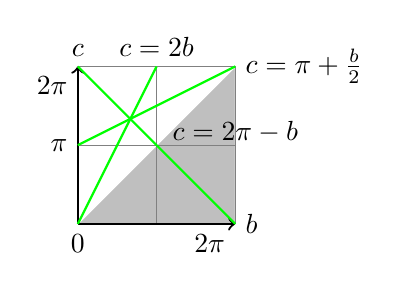
\begin{tikzpicture}
			\filldraw[fill=black!25, draw=black!0] (0,0) -- (2,2) -- (2,0) -- cycle;
			\draw[step=1cm,gray,very thin] (0,0) grid (2,2);
			\draw[thick,->] (0,0) node[anchor=north] {$0$} -- (2,0) node[anchor=west] {$b$} node[anchor=north east] {$2\pi$};
			\draw[thick,->] (0,0) -- (0,2) node[anchor=south] {$c$} node[anchor=north east] {$2\pi$};
			\draw[thick, green] (0,2) -- (2,0) node[above=9mm, black] {$c = 2\pi - b$};
			\draw[thick, green] (0,1) node[left, black] {$\pi$} -- (2,2) node[right, black] { $c = \pi + \frac{b}{2}$}; 
			\draw[thick, green] (0,0) -- (1,2) node[above, black] {$c = 2b$}; 
		\end{tikzpicture}
		$$
	\end{multicols}
	

	$$\mu(\Omega) = \frac{1}{2} (2\pi)^2 = 2\pi^2;\quad
	\mu(A) = \mu(\{c=\pi+\frac{b}{2}\} \cup \{c=2b\} \cup \{c=2\pi-b\}) = 0$$
	\begin{mdframed}[style=ans]
		$$P(A) = 0 $$
	\end{mdframed}
\end{enumerate}

\section*{№ 4.24}
\begin{mdframed}
	Олiвець довжиною l розламано навмання на три частини. 
	Знайдiть ймовiрнiсть того, що довжина середньої частини 
	виявиться \textbf{найменшою}.
\end{mdframed}

Тобто,
$$
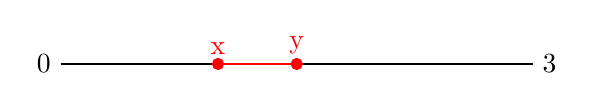
\begin{tikzpicture}
	\draw (0,0) node[left]{0} -- (6,0) node[right]{3};
	\draw[red] (1*2,0) -- (1.5*2,0);
	\filldraw[red] (1*2,0) circle (2pt) node[above] {x};
	\filldraw[red] (1.5*2,0) circle (2pt) node[above] {y};
\end{tikzpicture}
$$

Маємо:
$$ \Omega = \{(x,y) \in [0;3]^2 | x < y\};\quad x \in \Omega \text{ - координати точок розламу}$$
$$ \text{Подія } A = 
\left\{\begin{array}{c}
	y-x < x \\
	y-x < 3-y \\
	y > x
\end{array}\right. \implies
\left\{\begin{array}{c}
	y < 2x \\
	y < \frac{x}{2} + \frac{3}{2} \\
	y > x
\end{array}\right.$$
$$
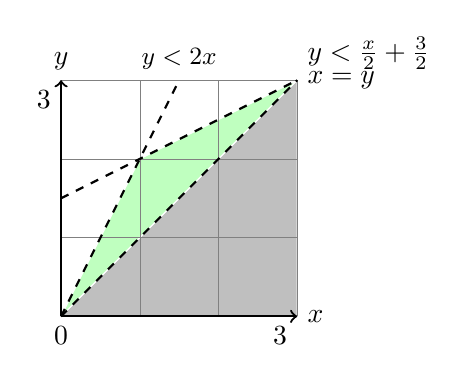
\begin{tikzpicture}
	\filldraw[fill=black!25, draw=black!0] (0,0) -- (3,3) -- (3,0) -- cycle;
	\filldraw[fill=green!25, draw=black!0] (0,0) -- (1,2) -- (3,3) -- cycle;
	\draw[step=1cm,gray,very thin] (0,0) grid (3,3);
	\draw[thick,->] (0,0) node[anchor=north] {$0$} -- (3,0) node[anchor=west] {$x$} node[anchor=north east] {$3$};
	\draw[thick,->] (0,0) -- (0,3) node[anchor=south] {$y$} node[anchor=north east] {$3$};
	\draw[thick, dashed] (0,0) -- (3,3) node[right] {$x = y$};
	\draw[thick, dashed] (0,0) -- (1.5,3) node[above] {\small $y < 2x$}; 
	\draw[thick, dashed] (0,1.5) -- (3,3) node[above right] {$y < \frac{x}{2} + \frac{3}{2}$}; 
\end{tikzpicture}
$$

$$\mu(\Omega) = \frac{1}{2} 3^2 = \frac{9}{2}$$
$$\mu(A) = \frac{1}{2} 1\cdot 1 + \frac{1}{2} 1 \cdot 2 = 1.5$$


\begin{mdframed}[style=ans]
	$$ P(A) = \frac{\mu(A)}{\mu(\Omega)} = \frac{3}{2} \cdot \frac{2}{9} = \frac{1}{3} $$
\end{mdframed}


\section*{№ 4.25}
\begin{mdframed}
	На паркет навмання кинуто монету радiусом 1 см. Знайдiть ймовiрнiсть того,
	що монета не перетне сторонiн паркету, якщо паркет має форму прямокутникiв
	зi сторонами 4 см i 8 см.
\end{mdframed}

Без обмеження загальності можна сказати, що центр монети потрапив в один з прямокутників.
Розглядатимимо положення монети в системі координат прямокутника, в який потрапив її центр.

$$
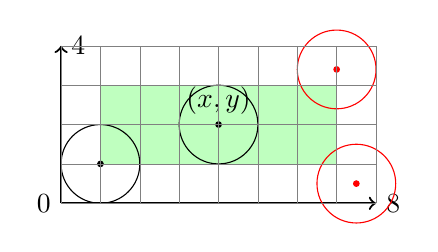
\begin{tikzpicture}
	% \draw[white] (0,0) -- (0,2) -- (4,2) -- (4,0) -- cycle;
	\filldraw[green!25] (0.5,0.5) -- (0.5,1.5) -- (3.5,1.5) -- (3.5,0.5) -- cycle;
	\draw[thick,->] (0,0) node[left]{0} -- (4,0) node[right]{8};
	\draw[thick,->] (0,0) -- (0,2) node[right]{4};
	\draw (0.5,0.5) circle (0.5);
	\filldraw (0.5,0.5) circle (1pt);
	\draw (2,1) circle (0.5) node[above ,black] {$(x,y)$};
	\filldraw (2,1) circle (1pt);
	\draw[red] (3.5,1.7) circle (0.5);
	\filldraw[red] (3.5,1.7) circle (1pt);
	\draw[red] (3.75,0.25) circle (0.5);
	\filldraw[red] (3.75,0.25) circle (1pt);
	\draw[step=0.5cm,gray,very thin] (0,0) grid (4,2);
\end{tikzpicture}
$$

Маємо:
$$ \Omega = [0;8]\times [0;4]; \quad (x,y) \in \Omega \text{ - координати центру монети}$$
$$ \text{Подія } A = [1;7] \times [1;3]$$

$$\mu(\Omega) = 8\cdot 4 = 32$$
$$\mu(A) = 6*2 = 12$$

\begin{mdframed}[style=ans]
	$$ P(A) = \frac{\mu(A)}{\mu(\Omega)} = \frac{12}{32} = \frac{3}{8} $$
\end{mdframed}